\documentclass[10pt,a4paper]{article}
\usepackage[utf8]{inputenc}
\usepackage[english]{babel}
\usepackage{amsmath}
\usepackage{amsfonts}
\usepackage{amssymb}
\usepackage{graphicx}
\usepackage[left=2cm,right=2cm,top=2cm,bottom=2cm]{geometry}
\usepackage{physics}
\usepackage{tikz}
\usepackage{stmaryrd}

\author{Marco Biroli}
\title{Graphene and Haldane model}

\begin{document}

\maketitle

\section{Graphene and Dirac points.}

\begin{enumerate}
\item  We have that:
\[
\vb{\delta_1} = (0, a) \mbox{~~and~~} \vb{\delta_2} = \frac{d}{2} (\sqrt{3}, -1) \mbox{~~and~~} \vb{\delta_3} = \frac{d}{2} (-\sqrt{3}, -1)
\]
Then we have that:
\begin{align*}
f_{\vb{k}} &= - t \exp(-\frac{i d}{2} (\sqrt{3} k_x + k_y)) \left( 1 + \exp(i \sqrt{3} d k_x) + \exp(\frac{i d}{2} (\sqrt{3} k_x + 3 k_y)) \right) \\
&= - t\left[ \underbrace{\left( 2 \cos(\frac{\sqrt{3}}{2} d k_x) \cos(\frac{d}{2} k_y) + \cos(d k_y) \right)}_{h_1} + i \underbrace{2 \left( \cos(\frac{\sqrt{3}}{2} d k_x) - \cos(\frac{d}{2} k_y) \right) \sin(\frac{d}{2} k_y)}_{h_2}
 \right]
\end{align*}
And taking $h_3 = 0$ we have that:
\[
H = -t \, \, \vb{h}_{\vb{k}} \cdot \vb{\sigma}
\]
Notice that without expanding the terms we can also simply write:
\[
H = \sum_{i = 1}^3 \left( \cos(\vb{k} \cdot \vb{\delta_i} ) \sigma_x + \sin(\vb{k} \cdot \vb{\delta_i}) \sigma_y \right)
\]
Then notice that similarly as in the TD we have that:
\[
H^2 = t^2 || \vb{h}_{\vb{k}} ||^2 \text{ Id}
\]
Thus the eigenvalues of $H$ are given by:
\[
E_\pm = \pm t || \vb{h_{\vb{k}}} || = \pm t \sqrt{3 + 2 \cos(d k_x \sqrt{3}) + 2 \cos(\frac{d}{2} (k_x\sqrt{3} - 3 k_y)) + 2 \cos(\frac{d}{2}(k_x\sqrt{3} + 3k_y))}
\]
Notice that solving for $E_\pm = 0$ we get indeed the Dirac point $K$, as well as $-K$ or $(K_x, - K_y)$ for example. Plotting the energy spectrum we obtain Figure \ref{eigenplot}.
\begin{figure}
\centering
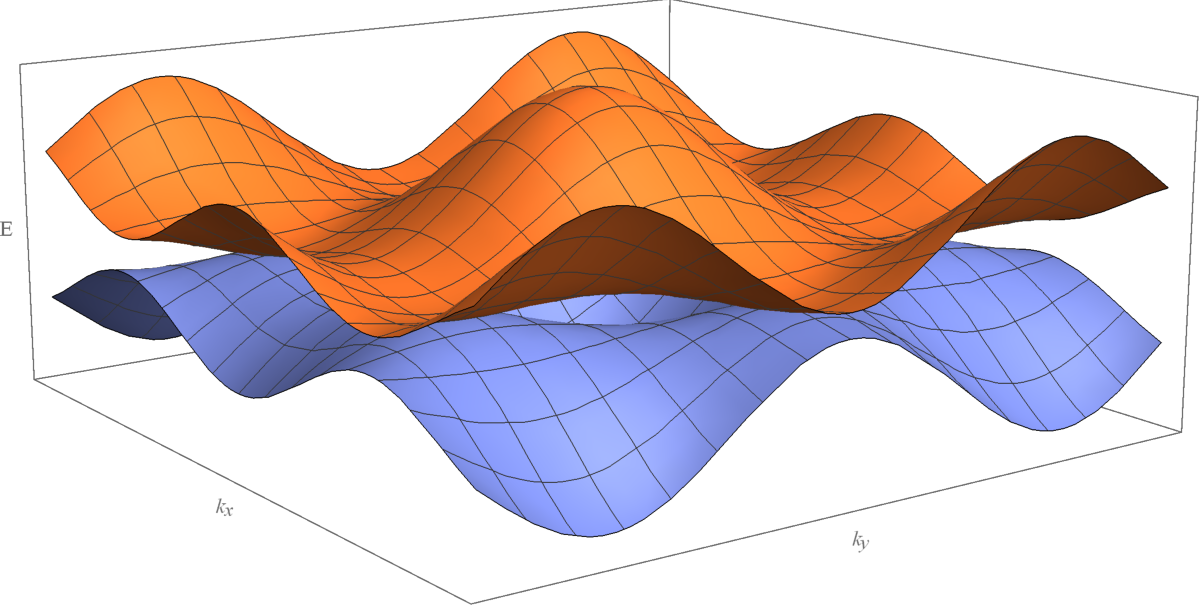
\includegraphics[width = 0.5\textwidth]{energylevels}
\caption{Plot of the positive energy levels for $k_x, k_y \in [-\frac{\pi}{d}, \frac{\pi}{d}]$.} \label{eigenplot}
\end{figure}

\item We write $\vb{k} = \vb{K} + \vb{\varepsilon}$. Then we know that $H_{\vb{K}} = 0$ and $f_{\vb{K}} = 0$ hence we have that:
\[
f_{\vb{k}} = f_{\vb{K}}  + \frac{1}{2}\vb{\varepsilon} \cdot \left(\grad f_{\vb{k}} \right) \Big|_{\vb{k} = \vb{K}} = \frac{1}{2} \vb{\varepsilon} \cdot \left( \frac{3 d t}{2}, - \frac{3}{2} i d t  \right) = \frac{3dt}{4}\left( \varepsilon_x - i \varepsilon_y \right)
\] 
Hence we also get the linearization of $\vb{h}$ easily as:
\[
\vb{h}_{\vb{k}} = \left(\frac{3dt}{4} (k_x - K_x), -\frac{3 dt}{4} (k_y - K_y)\right)  = \frac{3 dt}{4}\left(\varepsilon_x, - \varepsilon_y \right)
\]
And hence:
\[
E_\pm = \pm t \frac{3 dt}{4} \sqrt{\varepsilon_x^2 + \varepsilon_y^2} = \pm \frac{3 d t}{4} r 
\]

\item Close to $\vb{K}$ the Hamitlonian reads:
\[
H = \frac{3 d t}{4}\begin{pmatrix}
0 & \varepsilon_x + i \varepsilon_y\\
\varepsilon_x - i \varepsilon_y & 0 
\end{pmatrix}
\]
Hence we have that the eigenvectors are given by:
\[
u_{\pm \vb{k}} = \begin{pmatrix}
\pm \sqrt{\varepsilon_x^2 + \varepsilon_y^2}\\
\varepsilon_x - i \varepsilon_y
\end{pmatrix} = \begin{pmatrix}
\pm \varepsilon\\
\varepsilon e^{-i \theta}
\end{pmatrix} \propto \begin{pmatrix}
\pm e^{i \theta/2}\\
e^{-i\theta/2}
\end{pmatrix}
\]
Where we took:
\[
\cos \theta = \frac{\varepsilon_x}{\varepsilon} \mbox{~~and~~} \sin \theta = \frac{\varepsilon_y}{\varepsilon} \mbox{~~and~~} \varepsilon = \sqrt{\varepsilon_x^2 + \varepsilon_y^2}
\]
Now however notice that at the origin i.e. $\varepsilon_x = \varepsilon_y = 0$ we have that $\theta$ is not well defined. Now for the Berry connection we see that there is only an angular dependency hence we have:
\[
\mathcal{A}_{\pm} = i (u_{\pm}^T)^\star \cdot \grad u_{\pm} = \begin{pmatrix}
1 & e^{i\theta}
\end{pmatrix} \begin{pmatrix}
0\\
-i e^{-i \theta}
\end{pmatrix} =  \frac{1}{\varepsilon} \vu{\theta} 
\]

\item We then have that the Berry phase is going to be given by:
\[
\varphi_\mathcal{A} = \int_\mathcal{C} \vb{\mathcal{A}_\pm} \dd \vb{l} = \int_\mathcal{C} \frac{1}{\varepsilon} \dd \theta = 2 \pi n \mbox{~~with~~} n \in \mathbb{Z}
\]

\item We are now modifying $f_{\vb{k}}$ to:
\[
f'_{\vb{k}} = - t' e^{i \vb{k} \cdot \vb{\delta_1}} - t \sum_{i = 2}^3 e^{i \vb{k} \cdot \vb{\delta_i}}
\]
Which then gives for the energies:
\[
E'_\pm = \sqrt{2t^2 + t'^2 + 2t \left( t \cos(d k_x \sqrt{3}) + t'\left( \cos(\frac{d}{2} (k_x \sqrt{3} - 3 k_y)) + \cos(\frac{d}{2}(k_x\sqrt{3} + 3 k_y)) \right) \right)}
\]

\item Similarly as before by taking $\vb{k} = \vb{M} + \vb{\varepsilon}$ and making an expansion of $f'_{\vb{k}}$ we obtain:
\[
f'_{\vb{k}} \approx e^{i\frac{\pi}{6}} (2 i t - i t' + d(t + t')\varepsilon_y)
\]
Hence the Hamiltonian is given by:
\[
H = \begin{pmatrix}
0 & e^{- i \frac{\pi}{6}} (i t' - 2 i t + d(t + t')\varepsilon_y)\\
e^{i\frac{\pi}{6}} (2 i t - i t' + d(t + t')\varepsilon_y) & 0 
\end{pmatrix}
\]

\item See Figure \ref{fkvfield} 
\begin{figure} 
\centering
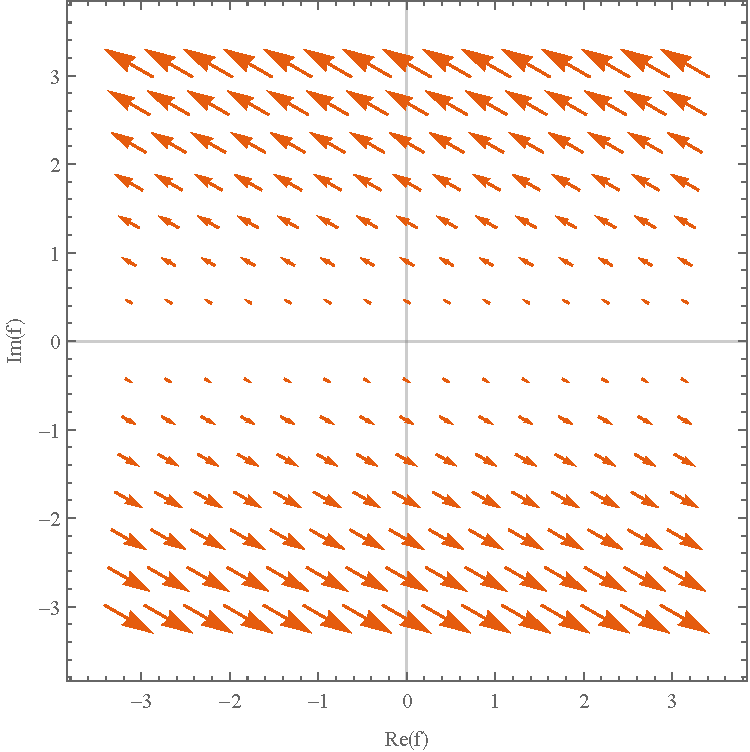
\includegraphics[width=0.5\textwidth]{fkvfield}
\caption{Orientation of $f(\vb{k})$} \label{fkvfield}
\end{figure}

\item 

\end{enumerate}

\section{The Haldane Model}

\begin{enumerate}

\item Cells can be indexed by two integers $(i, j)$ where the $i$ index corresponds to the horizontal position and the $j$ to the vertical position. Then we write the orbitals $\ket{i, j, A}$ and $\ket{i, j, B}$ for $A$ and $B$ respectively. Then the Hamiltonian is given by:
\begin{align*}
H = \sum_{i, j} &t\Big(\op{i, j, B}{i, j, A} + \op{i, j+1, B}{i, j, A} + \op{i+1, j, B}{i, j, A}\Big)\\
+ &t_2 e^{i\varphi}\Big(\op{i, j + 1, A}{i,j, A} + \op{i, j - 1, A}{i,j, A} + \op{i - 1, j, A}{i,j, A}\Big) + \frac{M}{2}\op{i, j, A}\\
+ &t_2 e^{-i\varphi}\Big(\op{i, j + 1, B}{i,j, B} + \op{i, j - 1, B}{i,j, B} + \op{i - 1, j, B}{i,j, B}\Big) - \frac{M}{2}\op{i, j, B}\\
+ &h.c.
\end{align*}

\item The first line and it's Hermitian conjugate of the above definition of the Hamiltonian corresponds to the one studied in part one and we will denote it by $H_0$ which we already know can be expressed as $H_0 = \vb{h} \cdot \vb{\sigma}$. Now we study the two remaining lines of the Hamiltonian. The first one (resp. second one) corresponds to the contribution from clock-wise hoping on $A-A$ terms plus the staggered potential (resp. $B-B$ terms with the staggered potential). Which we can re-write as:
\[
\ket{i,j, A} \left(\frac{M}{2} + t_2 e^{i\varphi} \sum_{j = 1}^3 e^{i \vb{k} \cdot \vb{b_j}}\right) \bra{i, j, A} \mbox{~~and~~} \ket{i, j, B} \left(\frac{-M}{2} + t_2 e^{-i \varphi} \sum_{j = 1}^3 e^{i \vb{k} \cdot \vb{b_j}} \right)\bra{i, j, B}
\]
Then adding these with their conjugates will give:
\[
\begin{pmatrix}
\ket{i, j, A} & \ket{i, j, B}
\end{pmatrix} \begin{pmatrix}
2 \Re\left( t_2 e^{i \varphi} \sum_{j = 1}^3 e^{i \vb{k} \cdot \vb{b_j}} \right) + M & 0\\
0 & 2 \Re\left( t_2 e^{-i\varphi} \sum_{j = 1}^3 e^{i \vb{k} \cdot \vb{b_j}} \right) - M
\end{pmatrix}
\begin{pmatrix}
\bra{i, j, A}\\
\bra{i, j, B}
\end{pmatrix}
\]
Now from the properties:
\[
\Re(a b) = \Re(a)\Re(b) - \Im(a)\Im(b) \mbox{~~and~~} \Re(a) = \Re(a^\star) \mbox{~~and~~} \Im(a) = -\Im(a^\star)
\]
We can simplify the above (calling $a = t_2e^{i \varphi}$ and $b$ the sum):
\begin{align*}
&\begin{pmatrix}
\ket{i, j, A} & \ket{i, j, B}
\end{pmatrix} \begin{pmatrix}
2 \Re\left( ab \right) + M & 0\\
0 & 2 \Re\left( a^\star b \right) - M
\end{pmatrix}
\begin{pmatrix}
\bra{i, j, A}\\
\bra{i, j, B}
\end{pmatrix}
\\
=
&\begin{pmatrix}
\ket{i, j, A} & \ket{i, j, B}
\end{pmatrix} \begin{pmatrix}
2 \Re(a)\Re(b) - 2 \Im(a) \Im(b) + M & 0\\
0 & 2 \Re(a^\star) \Re(b) - 2 \Im(a^\star) \Im(b) - M
\end{pmatrix}
\begin{pmatrix}
\bra{i, j, A}\\
\bra{i, j, B}
\end{pmatrix}
\\
=
&\begin{pmatrix}
\ket{i, j, A} & \ket{i, j, B}
\end{pmatrix} \begin{pmatrix}
2 \Re(a)\Re(b) + (-2 \Im(a) \Im(b) + M)& 0\\
0 & 2 \Re(a) \Re(b) - (-2 \Im(a) \Im(b) + M) 
\end{pmatrix}
\begin{pmatrix}
\bra{i, j, A}\\
\bra{i, j, B}
\end{pmatrix}
\\
=
&\begin{pmatrix}
\ket{i, j, A} & \ket{i, j, B}
\end{pmatrix} \Bigg(2 Re(a) Re(b) \text{Id} + \Big(M - 2 \Im(a) \Im(b) \Big) \sigma_z \Bigg)
\begin{pmatrix}
\bra{i, j, A}\\
\bra{i, j, B}
\end{pmatrix}
\end{align*}
Hence now we write:
\[
\varepsilon_0(\vb{k}) = 2 \Re(a) \Re(b) = 2 \cos\varphi \sum_{j = 1}^3 \cos(\vb{k} \cdot \vb{b_j})
\]
As well as:
\[
d_z(\vb{k}) = M - 2 \Im(a) \Im(b) = M - 2 t_2 \sin(\varphi) \sum_{j = 1}^3 \sin(\vb{k} \cdot \vb{b_j})
\]
Then we define:
\[
\vb{d}(\vb{k}) = \vb{h}(\vb{k}) + d_z(\vb{k}) \vu{z}
\]
Which allows us to re-write:
\[
H = \sum_{\vb{k}} \begin{pmatrix}
\ket{\vb{k}, A} & \ket{\vb{k}, B}
\end{pmatrix}
\underbrace{\Big( \varepsilon_0(\vb{k}) \text{Id} + \vb{d}(\vb{k}) \cdot \vb{\sigma} \Big)}_{H_{\vb{k}}} \begin{pmatrix}
\bra{\vb{k}, A}\\
\bra{\vb{k}, B}
\end{pmatrix}
\]

\item We have immediately that the eigenvalues of $H_{\vb{k}}$ are going to be given by:
\[
E_{\pm\vb{k}} = \varepsilon_0(\vb{k}) \pm ||\vb{d}(\vb{k})||
\]
Hence we have that:
\[
\Delta E_{\pm \vb{k}} = E_{+\vb{k}} - E_{-\vb{k}} = 2 ||d(\vb{k})||
\]
Hence gaps close if and only if:
\[
2||\vb{d}(\vb{k})|| = 0 \Leftrightarrow ||\vb{h}(\vb{k})||^2 + d_z(\vb{k})^2 = 0 \Leftrightarrow \begin{cases}
||h(\vb{k})||^2 = 0\\
d_z(\vb{k})^2 = 0
\end{cases} \Rightarrow d_z(\vb{K}) = 0
\]
Furthermore from the relation that we are given we have that:
\[
d_z(\vb{K}) = M + 3 t_2 \sin(\varphi)\sqrt{3}
\]

\item ...

\item 

\end{enumerate}

\end{document}